\documentclass[1p]{elsarticle_modified}
%\bibliographystyle{elsarticle-num}

%\usepackage[colorlinks]{hyperref}
%\usepackage{abbrmath_seonhwa} %\Abb, \Ascr, \Acal ,\Abf, \Afrak
\usepackage{amsfonts}
\usepackage{amssymb}
\usepackage{amsmath}
\usepackage{amsthm}
\usepackage{scalefnt}
\usepackage{amsbsy}
\usepackage{kotex}
\usepackage{caption}
\usepackage{subfig}
\usepackage{color}
\usepackage{graphicx}
\usepackage{xcolor} %% white, black, red, green, blue, cyan, magenta, yellow
\usepackage{float}
\usepackage{setspace}
\usepackage{hyperref}

\usepackage{tikz}
\usetikzlibrary{arrows}

\usepackage{multirow}
\usepackage{array} % fixed length table
\usepackage{hhline}

%%%%%%%%%%%%%%%%%%%%%
\makeatletter
\renewcommand*\env@matrix[1][\arraystretch]{%
	\edef\arraystretch{#1}%
	\hskip -\arraycolsep
	\let\@ifnextchar\new@ifnextchar
	\array{*\c@MaxMatrixCols c}}
\makeatother %https://tex.stackexchange.com/questions/14071/how-can-i-increase-the-line-spacing-in-a-matrix
%%%%%%%%%%%%%%%

\usepackage[normalem]{ulem}

\newcommand{\msout}[1]{\ifmmode\text{\sout{\ensuremath{#1}}}\else\sout{#1}\fi}
%SOURCE: \msout is \stkout macro in https://tex.stackexchange.com/questions/20609/strikeout-in-math-mode

\newcommand{\cancel}[1]{
	\ifmmode
	{\color{red}\msout{#1}}
	\else
	{\color{red}\sout{#1}}
	\fi
}

\newcommand{\add}[1]{
	{\color{blue}\uwave{#1}}
}

\newcommand{\replace}[2]{
	\ifmmode
	{\color{red}\msout{#1}}{\color{blue}\uwave{#2}}
	\else
	{\color{red}\sout{#1}}{\color{blue}\uwave{#2}}
	\fi
}

\newcommand{\Sol}{\mathcal{S}} %segment
\newcommand{\D}{D} %diagram
\newcommand{\A}{\mathcal{A}} %arc


%%%%%%%%%%%%%%%%%%%%%%%%%%%%%5 test

\def\sl{\operatorname{\textup{SL}}(2,\Cbb)}
\def\psl{\operatorname{\textup{PSL}}(2,\Cbb)}
\def\quan{\mkern 1mu \triangleright \mkern 1mu}

\theoremstyle{definition}
\newtheorem{thm}{Theorem}[section]
\newtheorem{prop}[thm]{Proposition}
\newtheorem{lem}[thm]{Lemma}
\newtheorem{ques}[thm]{Question}
\newtheorem{cor}[thm]{Corollary}
\newtheorem{defn}[thm]{Definition}
\newtheorem{exam}[thm]{Example}
\newtheorem{rmk}[thm]{Remark}
\newtheorem{alg}[thm]{Algorithm}

\newcommand{\I}{\sqrt{-1}}
\begin{document}

%\begin{frontmatter}
%
%\title{Boundary parabolic representations of knots up to 8 crossings}
%
%%% Group authors per affiliation:
%\author{Yunhi Cho} 
%\address{Department of Mathematics, University of Seoul, Seoul, Korea}
%\ead{yhcho@uos.ac.kr}
%
%
%\author{Seonhwa Kim} %\fnref{s_kim}}
%\address{Center for Geometry and Physics, Institute for Basic Science, Pohang, 37673, Korea}
%\ead{ryeona17@ibs.re.kr}
%
%\author{Hyuk Kim}
%\address{Department of Mathematical Sciences, Seoul National University, Seoul 08826, Korea}
%\ead{hyukkim@snu.ac.kr}
%
%\author{Seokbeom Yoon}
%\address{Department of Mathematical Sciences, Seoul National University, Seoul, 08826,  Korea}
%\ead{sbyoon15@snu.ac.kr}
%
%\begin{abstract}
%We find all boundary parabolic representation of knots up to 8 crossings.
%
%\end{abstract}
%\begin{keyword}
%    \MSC[2010] 57M25 
%\end{keyword}
%
%\end{frontmatter}

%\linenumbers
%\tableofcontents
%
\newcommand\colored[1]{\textcolor{white}{\rule[-0.35ex]{0.8em}{1.4ex}}\kern-0.8em\color{red} #1}%
%\newcommand\colored[1]{\textcolor{white}{ #1}\kern-2.17ex	\textcolor{white}{ #1}\kern-1.81ex	\textcolor{white}{ #1}\kern-2.15ex\color{red}#1	}

{\Large $\underline{11n_{69}~(K11n_{69})}$}

\setlength{\tabcolsep}{10pt}
\renewcommand{\arraystretch}{1.6}
\vspace{1cm}\begin{tabular}{m{100pt}>{\centering\arraybackslash}m{274pt}}
\multirow{5}{120pt}{
	\centering
	\includegraphics[width=112pt]{../../../GIT/diagram.site/Diagrams/png/685_11n_69.png}\\
\ \ \ A knot diagram\footnotemark}&
\allowdisplaybreaks
\textbf{Linearized knot diagam} \\
\cline{2-2}
 &
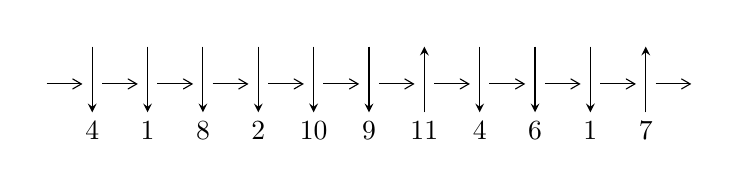
\begin{tikzpicture}[x=20pt, y=17pt]
	% nodes
	\node (C0) at (0, 0) {};
	\node (C1) at (1, 0) {};
	\node (C1U) at (1, +1) {};
	\node (C1D) at (1, -1) {4};

	\node (C2) at (2, 0) {};
	\node (C2U) at (2, +1) {};
	\node (C2D) at (2, -1) {1};

	\node (C3) at (3, 0) {};
	\node (C3U) at (3, +1) {};
	\node (C3D) at (3, -1) {8};

	\node (C4) at (4, 0) {};
	\node (C4U) at (4, +1) {};
	\node (C4D) at (4, -1) {2};

	\node (C5) at (5, 0) {};
	\node (C5U) at (5, +1) {};
	\node (C5D) at (5, -1) {10};

	\node (C6) at (6, 0) {};
	\node (C6U) at (6, +1) {};
	\node (C6D) at (6, -1) {9};

	\node (C7) at (7, 0) {};
	\node (C7U) at (7, +1) {};
	\node (C7D) at (7, -1) {11};

	\node (C8) at (8, 0) {};
	\node (C8U) at (8, +1) {};
	\node (C8D) at (8, -1) {4};

	\node (C9) at (9, 0) {};
	\node (C9U) at (9, +1) {};
	\node (C9D) at (9, -1) {6};

	\node (C10) at (10, 0) {};
	\node (C10U) at (10, +1) {};
	\node (C10D) at (10, -1) {1};

	\node (C11) at (11, 0) {};
	\node (C11U) at (11, +1) {};
	\node (C11D) at (11, -1) {7};
	\node (C12) at (12, 0) {};

	% arrows
	\draw[->,>={angle 60}]
	(C0) edge (C1) (C1) edge (C2) (C2) edge (C3) (C3) edge (C4) (C4) edge (C5) (C5) edge (C6) (C6) edge (C7) (C7) edge (C8) (C8) edge (C9) (C9) edge (C10) (C10) edge (C11) (C11) edge (C12) ;	\draw[->,>=stealth]
	(C1U) edge (C1D) (C2U) edge (C2D) (C3U) edge (C3D) (C4U) edge (C4D) (C5U) edge (C5D) (C6U) edge (C6D) (C7D) edge (C7U) (C8U) edge (C8D) (C9U) edge (C9D) (C10U) edge (C10D) (C11D) edge (C11U) ;
	\end{tikzpicture} \\
\hhline{~~} \\& 
\textbf{Solving Sequence} \\ \cline{2-2} 
 &
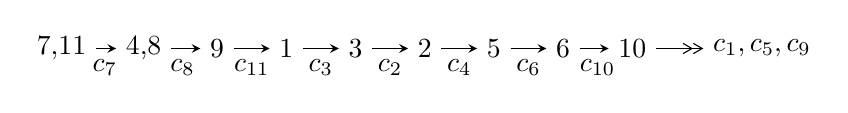
\begin{tikzpicture}[x=25pt, y=7pt]
	% node
	\node (A0) at (-1/8, 0) {7,11};
	\node (A1) at (17/16, 0) {4,8};
	\node (A2) at (17/8, 0) {9};
	\node (A3) at (25/8, 0) {1};
	\node (A4) at (33/8, 0) {3};
	\node (A5) at (41/8, 0) {2};
	\node (A6) at (49/8, 0) {5};
	\node (A7) at (57/8, 0) {6};
	\node (A8) at (65/8, 0) {10};
	\node (C1) at (1/2, -1) {$c_{7}$};
	\node (C2) at (13/8, -1) {$c_{8}$};
	\node (C3) at (21/8, -1) {$c_{11}$};
	\node (C4) at (29/8, -1) {$c_{3}$};
	\node (C5) at (37/8, -1) {$c_{2}$};
	\node (C6) at (45/8, -1) {$c_{4}$};
	\node (C7) at (53/8, -1) {$c_{6}$};
	\node (C8) at (61/8, -1) {$c_{10}$};
	\node (A9) at (10, 0) {$c_{1},c_{5},c_{9}$};

	% edge
	\draw[->,>=stealth]	
	(A0) edge (A1) (A1) edge (A2) (A2) edge (A3) (A3) edge (A4) (A4) edge (A5) (A5) edge (A6) (A6) edge (A7) (A7) edge (A8) ;
	\draw[->>,>={angle 60}]	
	(A8) edge (A9);
\end{tikzpicture} \\ 

\end{tabular} \\

\footnotetext{
The image of knot diagram is generated by the software ``\textbf{Draw programme}" developed by Andrew Bartholomew(\url{http://www.layer8.co.uk/maths/draw/index.htm\#Running-draw}), where we modified some parts for our purpose(\url{https://github.com/CATsTAILs/LinksPainter}).
}\phantom \\ \newline 
\centering \textbf{Ideals for irreducible components\footnotemark of $X_{\text{par}}$} 
 
\begin{align*}
I^u_{1}&=\langle 
3951 u^{19}+6529 u^{18}+\cdots+2424 b+6325,\;-115811 u^{19}-169485 u^{18}+\cdots+79992 a-272713,\\
\phantom{I^u_{1}}&\phantom{= \langle  }u^{20}+2 u^{19}+\cdots+2 u+1\rangle \\
I^u_{2}&=\langle 
u^3+2 b- u+1,\;- u^3+2 u^2+2 a-3 u+1,\;u^4- u^3+u^2+1\rangle \\
I^u_{3}&=\langle 
u^5+u^4+u^3- u^2+b-2 u,\;u^4- u^3+u^2+a-3 u+2,\;u^6+2 u^4-3 u^3+u^2-3 u+1\rangle \\
\\
\end{align*}
\raggedright * 3 irreducible components of $\dim_{\mathbb{C}}=0$, with total 30 representations.\\
\footnotetext{All coefficients of polynomials are rational numbers. But the coefficients are sometimes approximated in decimal forms when there is not enough margin.}
\newpage
\renewcommand{\arraystretch}{1}
\centering \section*{I. $I^u_{1}= \langle 3951 u^{19}+6529 u^{18}+\cdots+2424 b+6325,\;-1.16\times10^{5} u^{19}-1.69\times10^{5} u^{18}+\cdots+8.00\times10^{4} a-2.73\times10^{5},\;u^{20}+2 u^{19}+\cdots+2 u+1 \rangle$}
\flushleft \textbf{(i) Arc colorings}\\
\begin{tabular}{m{7pt} m{180pt} m{7pt} m{180pt} }
\flushright $a_{7}=$&$\begin{pmatrix}1\\0\end{pmatrix}$ \\
\flushright $a_{11}=$&$\begin{pmatrix}0\\u\end{pmatrix}$ \\
\flushright $a_{4}=$&$\begin{pmatrix}1.44778 u^{19}+2.11877 u^{18}+\cdots+7.14120 u+3.40925\\-1.62995 u^{19}-2.69348 u^{18}+\cdots+1.21988 u-2.60932\end{pmatrix}$ \\
\flushright $a_{8}=$&$\begin{pmatrix}1\\- u^2\end{pmatrix}$ \\
\flushright $a_{9}=$&$\begin{pmatrix}-0.490249 u^{19}-0.377738 u^{18}+\cdots+1.43684 u-0.710171\\2.45375 u^{19}+3.57816 u^{18}+\cdots+2.48335 u+4.64226\end{pmatrix}$ \\
\flushright $a_{1}=$&$\begin{pmatrix}u\\u\end{pmatrix}$ \\
\flushright $a_{3}=$&$\begin{pmatrix}0.315419 u^{19}+0.424955 u^{18}+\cdots+8.46688 u+1.57672\\-1.38148 u^{19}-2.28739 u^{18}+\cdots+1.22934 u-2.03842\end{pmatrix}$ \\
\flushright $a_{2}=$&$\begin{pmatrix}-0.349372 u^{19}-0.474610 u^{18}+\cdots+8.80089 u+0.895277\\-2.04627 u^{19}-3.18696 u^{18}+\cdots+1.56334 u-2.71986\end{pmatrix}$ \\
\flushright $a_{5}=$&$\begin{pmatrix}3.68497 u^{19}+5.12691 u^{18}+\cdots-2.11341 u+4.48245\\-0.354535 u^{19}-0.633363 u^{18}+\cdots-0.327633 u-1.82848\end{pmatrix}$ \\
\flushright $a_{6}=$&$\begin{pmatrix}-4.03950 u^{19}-5.76028 u^{18}+\cdots+1.78578 u-5.31093\\-1.32933 u^{19}-1.83018 u^{18}+\cdots-0.265227 u-1.45375\end{pmatrix}$ \\
\flushright $a_{10}=$&$\begin{pmatrix}u^3\\u^3+u\end{pmatrix}$\\ \flushright $a_{10}=$&$\begin{pmatrix}u^3\\u^3+u\end{pmatrix}$\\&\end{tabular}
\flushleft \textbf{(ii) Obstruction class $= -1$}\\~\\
\flushleft \textbf{(iii) Cusp Shapes $= \frac{189289}{17776} u^{19}+\frac{857557}{53328} u^{18}+\cdots+\frac{286735}{53328} u+\frac{706201}{53328}$}\\~\\
\newpage\renewcommand{\arraystretch}{1}
\flushleft \textbf{(iv) u-Polynomials at the component}\newline \\
\begin{tabular}{m{50pt}|m{274pt}}
Crossings & \hspace{64pt}u-Polynomials at each crossing \\
\hline $$\begin{aligned}c_{1},c_{4}\end{aligned}$$&$\begin{aligned}
&u^{20}-2 u^{19}+\cdots-35 u+4
\end{aligned}$\\
\hline $$\begin{aligned}c_{2}\end{aligned}$$&$\begin{aligned}
&u^{20}+22 u^{19}+\cdots+353 u+16
\end{aligned}$\\
\hline $$\begin{aligned}c_{3},c_{8}\end{aligned}$$&$\begin{aligned}
&u^{20}+2 u^{19}+\cdots+112 u+64
\end{aligned}$\\
\hline $$\begin{aligned}c_{5},c_{6},c_{9}\end{aligned}$$&$\begin{aligned}
&u^{20}-2 u^{19}+\cdots-2 u+1
\end{aligned}$\\
\hline $$\begin{aligned}c_{7},c_{11}\end{aligned}$$&$\begin{aligned}
&u^{20}-2 u^{19}+\cdots-2 u+1
\end{aligned}$\\
\hline $$\begin{aligned}c_{10}\end{aligned}$$&$\begin{aligned}
&u^{20}+14 u^{19}+\cdots+4 u+1
\end{aligned}$\\
\hline
\end{tabular}\\~\\
\newpage\renewcommand{\arraystretch}{1}
\flushleft \textbf{(v) Riley Polynomials at the component}\newline \\
\begin{tabular}{m{50pt}|m{274pt}}
Crossings & \hspace{64pt}Riley Polynomials at each crossing \\
\hline $$\begin{aligned}c_{1},c_{4}\end{aligned}$$&$\begin{aligned}
&y^{20}-22 y^{19}+\cdots-353 y+16
\end{aligned}$\\
\hline $$\begin{aligned}c_{2}\end{aligned}$$&$\begin{aligned}
&y^{20}-46 y^{19}+\cdots+223775 y+256
\end{aligned}$\\
\hline $$\begin{aligned}c_{3},c_{8}\end{aligned}$$&$\begin{aligned}
&y^{20}-18 y^{19}+\cdots+45824 y+4096
\end{aligned}$\\
\hline $$\begin{aligned}c_{5},c_{6},c_{9}\end{aligned}$$&$\begin{aligned}
&y^{20}+14 y^{19}+\cdots+4 y+1
\end{aligned}$\\
\hline $$\begin{aligned}c_{7},c_{11}\end{aligned}$$&$\begin{aligned}
&y^{20}+14 y^{19}+\cdots+4 y+1
\end{aligned}$\\
\hline $$\begin{aligned}c_{10}\end{aligned}$$&$\begin{aligned}
&y^{20}-14 y^{19}+\cdots+56 y+1
\end{aligned}$\\
\hline
\end{tabular}\\~\\
\newpage\flushleft \textbf{(vi) Complex Volumes and Cusp Shapes}
$$\begin{array}{c|c|c}  
\text{Solutions to }I^u_{1}& \I (\text{vol} + \sqrt{-1}CS) & \text{Cusp shape}\\
 \hline 
\begin{aligned}
u &= -1.131630 + 0.044257 I \\
a &= \phantom{-}0.0439473 + 0.1087160 I \\
b &= \phantom{-}1.40407 + 0.37862 I\end{aligned}
 & -4.62345 - 6.11364 I & -7.31633 + 3.70196 I \\ \hline\begin{aligned}
u &= -1.131630 - 0.044257 I \\
a &= \phantom{-}0.0439473 - 0.1087160 I \\
b &= \phantom{-}1.40407 - 0.37862 I\end{aligned}
 & -4.62345 + 6.11364 I & -7.31633 - 3.70196 I \\ \hline\begin{aligned}
u &= -0.280810 + 0.786452 I \\
a &= -0.395074 + 0.246972 I \\
b &= -0.197007 + 0.388860 I\end{aligned}
 & -0.440396 - 1.279690 I & -4.66436 + 4.97948 I \\ \hline\begin{aligned}
u &= -0.280810 - 0.786452 I \\
a &= -0.395074 - 0.246972 I \\
b &= -0.197007 - 0.388860 I\end{aligned}
 & -0.440396 + 1.279690 I & -4.66436 - 4.97948 I \\ \hline\begin{aligned}
u &= \phantom{-}0.769131 + 0.907087 I \\
a &= \phantom{-}0.304381 - 0.204058 I \\
b &= -0.165796 + 0.163987 I\end{aligned}
 & \phantom{-}5.68828 + 2.93127 I & \phantom{-}2.45037 - 0.45578 I \\ \hline\begin{aligned}
u &= \phantom{-}0.769131 - 0.907087 I \\
a &= \phantom{-}0.304381 + 0.204058 I \\
b &= -0.165796 - 0.163987 I\end{aligned}
 & \phantom{-}5.68828 - 2.93127 I & \phantom{-}2.45037 + 0.45578 I \\ \hline\begin{aligned}
u &= \phantom{-}0.167664 + 1.190790 I \\
a &= \phantom{-}1.75974 + 0.44692 I \\
b &= \phantom{-}1.243080 - 0.457519 I\end{aligned}
 & -4.30761 + 1.95796 I & -13.39097 - 1.55059 I \\ \hline\begin{aligned}
u &= \phantom{-}0.167664 - 1.190790 I \\
a &= \phantom{-}1.75974 - 0.44692 I \\
b &= \phantom{-}1.243080 + 0.457519 I\end{aligned}
 & -4.30761 - 1.95796 I & -13.39097 + 1.55059 I \\ \hline\begin{aligned}
u &= \phantom{-}0.050177 + 1.253190 I \\
a &= \phantom{-}0.722975 + 0.985298 I \\
b &= \phantom{-}0.495740 - 0.417798 I\end{aligned}
 & -5.41434 + 1.81549 I & -13.14101 - 3.54833 I \\ \hline\begin{aligned}
u &= \phantom{-}0.050177 - 1.253190 I \\
a &= \phantom{-}0.722975 - 0.985298 I \\
b &= \phantom{-}0.495740 + 0.417798 I\end{aligned}
 & -5.41434 - 1.81549 I & -13.14101 + 3.54833 I\\
 \hline 
 \end{array}$$\newpage$$\begin{array}{c|c|c}  
\text{Solutions to }I^u_{1}& \I (\text{vol} + \sqrt{-1}CS) & \text{Cusp shape}\\
 \hline 
\begin{aligned}
u &= -0.261687 + 1.231270 I \\
a &= -2.05611 + 0.13028 I \\
b &= -1.122580 - 0.533009 I\end{aligned}
 & -2.03730 - 5.64317 I & -8.76092 + 6.80873 I \\ \hline\begin{aligned}
u &= -0.261687 - 1.231270 I \\
a &= -2.05611 - 0.13028 I \\
b &= -1.122580 + 0.533009 I\end{aligned}
 & -2.03730 + 5.64317 I & -8.76092 - 6.80873 I \\ \hline\begin{aligned}
u &= -0.553404 + 0.030516 I \\
a &= -0.394310 + 0.673104 I \\
b &= -0.895721 - 0.664676 I\end{aligned}
 & \phantom{-}1.73140 - 2.57417 I & -2.05095 + 4.12677 I \\ \hline\begin{aligned}
u &= -0.553404 - 0.030516 I \\
a &= -0.394310 - 0.673104 I \\
b &= -0.895721 + 0.664676 I\end{aligned}
 & \phantom{-}1.73140 + 2.57417 I & -2.05095 - 4.12677 I \\ \hline\begin{aligned}
u &= -0.52166 + 1.39992 I \\
a &= \phantom{-}1.63987 - 0.44598 I \\
b &= \phantom{-}1.74672 + 0.69883 I\end{aligned}
 & -9.1950 - 11.9560 I & -9.10352 + 6.09824 I \\ \hline\begin{aligned}
u &= -0.52166 - 1.39992 I \\
a &= \phantom{-}1.63987 + 0.44598 I \\
b &= \phantom{-}1.74672 - 0.69883 I\end{aligned}
 & -9.1950 + 11.9560 I & -9.10352 - 6.09824 I \\ \hline\begin{aligned}
u &= \phantom{-}0.54264 + 1.40344 I \\
a &= -1.38809 - 0.74127 I \\
b &= -1.65276 + 0.37354 I\end{aligned}
 & -13.3225 + 5.9895 I & -12.03384 - 3.05262 I \\ \hline\begin{aligned}
u &= \phantom{-}0.54264 - 1.40344 I \\
a &= -1.38809 + 0.74127 I \\
b &= -1.65276 - 0.37354 I\end{aligned}
 & -13.3225 - 5.9895 I & -12.03384 + 3.05262 I \\ \hline\begin{aligned}
u &= \phantom{-}0.219579 + 0.305083 I \\
a &= -0.48733 + 3.67126 I \\
b &= \phantom{-}0.894252 + 0.888486 I\end{aligned}
 & -0.977750 + 0.984957 I & -3.11347 + 0.07087 I \\ \hline\begin{aligned}
u &= \phantom{-}0.219579 - 0.305083 I \\
a &= -0.48733 - 3.67126 I \\
b &= \phantom{-}0.894252 - 0.888486 I\end{aligned}
 & -0.977750 - 0.984957 I & -3.11347 - 0.07087 I\\
 \hline 
 \end{array}$$\newpage\newpage\renewcommand{\arraystretch}{1}
\centering \section*{II. $I^u_{2}= \langle u^3+2 b- u+1,\;- u^3+2 u^2+2 a-3 u+1,\;u^4- u^3+u^2+1 \rangle$}
\flushleft \textbf{(i) Arc colorings}\\
\begin{tabular}{m{7pt} m{180pt} m{7pt} m{180pt} }
\flushright $a_{7}=$&$\begin{pmatrix}1\\0\end{pmatrix}$ \\
\flushright $a_{11}=$&$\begin{pmatrix}0\\u\end{pmatrix}$ \\
\flushright $a_{4}=$&$\begin{pmatrix}\frac{1}{2} u^3- u^2+\frac{3}{2} u-\frac{1}{2}\\-\frac{1}{2} u^3+\frac{1}{2} u-\frac{1}{2}\end{pmatrix}$ \\
\flushright $a_{8}=$&$\begin{pmatrix}1\\- u^2\end{pmatrix}$ \\
\flushright $a_{9}=$&$\begin{pmatrix}1\\- u^2\end{pmatrix}$ \\
\flushright $a_{1}=$&$\begin{pmatrix}u\\u\end{pmatrix}$ \\
\flushright $a_{3}=$&$\begin{pmatrix}\frac{1}{2} u^3- u^2+\frac{3}{2} u-\frac{1}{2}\\-\frac{1}{2} u^3+\frac{1}{2} u-\frac{1}{2}\end{pmatrix}$ \\
\flushright $a_{2}=$&$\begin{pmatrix}\frac{1}{2} u^3- u^2+\frac{5}{2} u-\frac{1}{2}\\-\frac{1}{2} u^3+\frac{3}{2} u-\frac{1}{2}\end{pmatrix}$ \\
\flushright $a_{5}=$&$\begin{pmatrix}- u\\- u\end{pmatrix}$ \\
\flushright $a_{6}=$&$\begin{pmatrix}u^2+1\\- u^3+u^2+1\end{pmatrix}$ \\
\flushright $a_{10}=$&$\begin{pmatrix}u^3\\u^3+u\end{pmatrix}$\\ \flushright $a_{10}=$&$\begin{pmatrix}u^3\\u^3+u\end{pmatrix}$\\&\end{tabular}
\flushleft \textbf{(ii) Obstruction class $= 1$}\\~\\
\flushleft \textbf{(iii) Cusp Shapes $= -\frac{1}{4} u^3-\frac{9}{2} u^2+\frac{9}{4} u-\frac{53}{4}$}\\~\\
\newpage\renewcommand{\arraystretch}{1}
\flushleft \textbf{(iv) u-Polynomials at the component}\newline \\
\begin{tabular}{m{50pt}|m{274pt}}
Crossings & \hspace{64pt}u-Polynomials at each crossing \\
\hline $$\begin{aligned}c_{1}\end{aligned}$$&$\begin{aligned}
&(u-1)^4
\end{aligned}$\\
\hline $$\begin{aligned}c_{2},c_{4}\end{aligned}$$&$\begin{aligned}
&(u+1)^4
\end{aligned}$\\
\hline $$\begin{aligned}c_{3},c_{8}\end{aligned}$$&$\begin{aligned}
&u^4
\end{aligned}$\\
\hline $$\begin{aligned}c_{5},c_{6},c_{10}\end{aligned}$$&$\begin{aligned}
&u^4- u^3+3 u^2-2 u+1
\end{aligned}$\\
\hline $$\begin{aligned}c_{7}\end{aligned}$$&$\begin{aligned}
&u^4- u^3+u^2+1
\end{aligned}$\\
\hline $$\begin{aligned}c_{9}\end{aligned}$$&$\begin{aligned}
&u^4+u^3+3 u^2+2 u+1
\end{aligned}$\\
\hline $$\begin{aligned}c_{11}\end{aligned}$$&$\begin{aligned}
&u^4+u^3+u^2+1
\end{aligned}$\\
\hline
\end{tabular}\\~\\
\newpage\renewcommand{\arraystretch}{1}
\flushleft \textbf{(v) Riley Polynomials at the component}\newline \\
\begin{tabular}{m{50pt}|m{274pt}}
Crossings & \hspace{64pt}Riley Polynomials at each crossing \\
\hline $$\begin{aligned}c_{1},c_{2},c_{4}\end{aligned}$$&$\begin{aligned}
&(y-1)^4
\end{aligned}$\\
\hline $$\begin{aligned}c_{3},c_{8}\end{aligned}$$&$\begin{aligned}
&y^4
\end{aligned}$\\
\hline $$\begin{aligned}c_{5},c_{6},c_{9}\\c_{10}\end{aligned}$$&$\begin{aligned}
&y^4+5 y^3+7 y^2+2 y+1
\end{aligned}$\\
\hline $$\begin{aligned}c_{7},c_{11}\end{aligned}$$&$\begin{aligned}
&y^4+y^3+3 y^2+2 y+1
\end{aligned}$\\
\hline
\end{tabular}\\~\\
\newpage\flushleft \textbf{(vi) Complex Volumes and Cusp Shapes}
$$\begin{array}{c|c|c}  
\text{Solutions to }I^u_{2}& \I (\text{vol} + \sqrt{-1}CS) & \text{Cusp shape}\\
 \hline 
\begin{aligned}
u &= -0.351808 + 0.720342 I \\
a &= -0.38053 + 1.53420 I \\
b &= -0.927958 + 0.413327 I\end{aligned}
 & -1.85594 - 1.41510 I & -12.38954 + 3.92814 I \\ \hline\begin{aligned}
u &= -0.351808 - 0.720342 I \\
a &= -0.38053 - 1.53420 I \\
b &= -0.927958 - 0.413327 I\end{aligned}
 & -1.85594 + 1.41510 I & -12.38954 - 3.92814 I \\ \hline\begin{aligned}
u &= \phantom{-}0.851808 + 0.911292 I \\
a &= \phantom{-}0.130534 + 0.427872 I \\
b &= \phantom{-}0.677958 - 0.157780 I\end{aligned}
 & \phantom{-}5.14581 + 3.16396 I & -10.48546 - 5.24252 I \\ \hline\begin{aligned}
u &= \phantom{-}0.851808 - 0.911292 I \\
a &= \phantom{-}0.130534 - 0.427872 I \\
b &= \phantom{-}0.677958 + 0.157780 I\end{aligned}
 & \phantom{-}5.14581 - 3.16396 I & -10.48546 + 5.24252 I\\
 \hline 
 \end{array}$$\newpage\newpage\renewcommand{\arraystretch}{1}
\centering \section*{III. $I^u_{3}= \langle u^5+u^4+u^3- u^2+b-2 u,\;u^4- u^3+u^2+a-3 u+2,\;u^6+2 u^4-3 u^3+u^2-3 u+1 \rangle$}
\flushleft \textbf{(i) Arc colorings}\\
\begin{tabular}{m{7pt} m{180pt} m{7pt} m{180pt} }
\flushright $a_{7}=$&$\begin{pmatrix}1\\0\end{pmatrix}$ \\
\flushright $a_{11}=$&$\begin{pmatrix}0\\u\end{pmatrix}$ \\
\flushright $a_{4}=$&$\begin{pmatrix}- u^4+u^3- u^2+3 u-2\\- u^5- u^4- u^3+u^2+2 u\end{pmatrix}$ \\
\flushright $a_{8}=$&$\begin{pmatrix}1\\- u^2\end{pmatrix}$ \\
\flushright $a_{9}=$&$\begin{pmatrix}u\\u\end{pmatrix}$ \\
\flushright $a_{1}=$&$\begin{pmatrix}u\\u\end{pmatrix}$ \\
\flushright $a_{3}=$&$\begin{pmatrix}- u^4- u^2+2 u-1\\- u^4+2 u\end{pmatrix}$ \\
\flushright $a_{2}=$&$\begin{pmatrix}2 u-1\\u^2+2 u\end{pmatrix}$ \\
\flushright $a_{5}=$&$\begin{pmatrix}u^4+u^2-1\\u^4+2 u^2\end{pmatrix}$ \\
\flushright $a_{6}=$&$\begin{pmatrix}- u^2+1\\- u^2\end{pmatrix}$ \\
\flushright $a_{10}=$&$\begin{pmatrix}u^3\\u^3+u\end{pmatrix}$\\ \flushright $a_{10}=$&$\begin{pmatrix}u^3\\u^3+u\end{pmatrix}$\\&\end{tabular}
\flushleft \textbf{(ii) Obstruction class $= -1$}\\~\\
\flushleft \textbf{(iii) Cusp Shapes $= -10$}\\~\\
\newpage\renewcommand{\arraystretch}{1}
\flushleft \textbf{(iv) u-Polynomials at the component}\newline \\
\begin{tabular}{m{50pt}|m{274pt}}
Crossings & \hspace{64pt}u-Polynomials at each crossing \\
\hline $$\begin{aligned}c_{1},c_{3},c_{4}\\c_{8}\end{aligned}$$&$\begin{aligned}
&(u^2- u-1)^3
\end{aligned}$\\
\hline $$\begin{aligned}c_{2}\end{aligned}$$&$\begin{aligned}
&(u^2+3 u+1)^3
\end{aligned}$\\
\hline $$\begin{aligned}c_{5},c_{6},c_{7}\\c_{9},c_{11}\end{aligned}$$&$\begin{aligned}
&u^6+2 u^4+3 u^3+u^2+3 u+1
\end{aligned}$\\
\hline $$\begin{aligned}c_{10}\end{aligned}$$&$\begin{aligned}
&u^6+4 u^5+6 u^4-3 u^3-13 u^2-7 u+1
\end{aligned}$\\
\hline
\end{tabular}\\~\\
\newpage\renewcommand{\arraystretch}{1}
\flushleft \textbf{(v) Riley Polynomials at the component}\newline \\
\begin{tabular}{m{50pt}|m{274pt}}
Crossings & \hspace{64pt}Riley Polynomials at each crossing \\
\hline $$\begin{aligned}c_{1},c_{3},c_{4}\\c_{8}\end{aligned}$$&$\begin{aligned}
&(y^2-3 y+1)^3
\end{aligned}$\\
\hline $$\begin{aligned}c_{2}\end{aligned}$$&$\begin{aligned}
&(y^2-7 y+1)^3
\end{aligned}$\\
\hline $$\begin{aligned}c_{5},c_{6},c_{7}\\c_{9},c_{11}\end{aligned}$$&$\begin{aligned}
&y^6+4 y^5+6 y^4-3 y^3-13 y^2-7 y+1
\end{aligned}$\\
\hline $$\begin{aligned}c_{10}\end{aligned}$$&$\begin{aligned}
&y^6-4 y^5+34 y^4-107 y^3+139 y^2-75 y+1
\end{aligned}$\\
\hline
\end{tabular}\\~\\
\newpage\flushleft \textbf{(vi) Complex Volumes and Cusp Shapes}
$$\begin{array}{c|c|c}  
\text{Solutions to }I^u_{3}& \I (\text{vol} + \sqrt{-1}CS) & \text{Cusp shape}\\
 \hline 
\begin{aligned}
u &= -0.170987 + 1.042930 I \\
a &= -1.89470 + 1.68750 I \\
b &= -1.98931 + 1.11042 I\end{aligned}
 & -0.986960\phantom{ +0.000000I} & -10.0000\phantom{ +0.000000I} \\ \hline\begin{aligned}
u &= -0.170987 - 1.042930 I \\
a &= -1.89470 - 1.68750 I \\
b &= -1.98931 - 1.11042 I\end{aligned}
 & -0.986960\phantom{ +0.000000I} & -10.0000\phantom{ +0.000000I} \\ \hline\begin{aligned}
u &= \phantom{-}1.13928\phantom{ +0.000000I} \\
a &= -0.0860817\phantom{ +0.000000I} \\
b &= -1.50630\phantom{ +0.000000I}\end{aligned}
 & -8.88264\phantom{ +0.000000I} & -10.0000\phantom{ +0.000000I} \\ \hline\begin{aligned}
u &= -0.56964 + 1.40480 I \\
a &= \phantom{-}0.970092 - 0.868217 I \\
b &= \phantom{-}1.371190 + 0.120928 I\end{aligned}
 & -8.88264\phantom{ +0.000000I} & -10.0000\phantom{ +0.000000I} \\ \hline\begin{aligned}
u &= -0.56964 - 1.40480 I \\
a &= \phantom{-}0.970092 + 0.868217 I \\
b &= \phantom{-}1.371190 - 0.120928 I\end{aligned}
 & -8.88264\phantom{ +0.000000I} & -10.0000\phantom{ +0.000000I} \\ \hline\begin{aligned}
u &= \phantom{-}0.341974\phantom{ +0.000000I} \\
a &= -1.06471\phantom{ +0.000000I} \\
b &= \phantom{-}0.742547\phantom{ +0.000000I}\end{aligned}
 & -0.986960\phantom{ +0.000000I} & -10.0000\phantom{ +0.000000I}\\
 \hline 
 \end{array}$$\newpage
\newpage\renewcommand{\arraystretch}{1}
\centering \section*{ IV. u-Polynomials}
\begin{tabular}{m{50pt}|m{274pt}}
Crossings & \hspace{64pt}u-Polynomials at each crossing \\
\hline $$\begin{aligned}c_{1}\end{aligned}$$&$\begin{aligned}
&((u-1)^4)(u^2- u-1)^3(u^{20}-2 u^{19}+\cdots-35 u+4)
\end{aligned}$\\
\hline $$\begin{aligned}c_{2}\end{aligned}$$&$\begin{aligned}
&((u+1)^4)(u^2+3 u+1)^3(u^{20}+22 u^{19}+\cdots+353 u+16)
\end{aligned}$\\
\hline $$\begin{aligned}c_{3},c_{8}\end{aligned}$$&$\begin{aligned}
&u^4(u^2- u-1)^3(u^{20}+2 u^{19}+\cdots+112 u+64)
\end{aligned}$\\
\hline $$\begin{aligned}c_{4}\end{aligned}$$&$\begin{aligned}
&((u+1)^4)(u^2- u-1)^3(u^{20}-2 u^{19}+\cdots-35 u+4)
\end{aligned}$\\
\hline $$\begin{aligned}c_{5},c_{6}\end{aligned}$$&$\begin{aligned}
&(u^4- u^3+3 u^2-2 u+1)(u^6+2 u^4+3 u^3+u^2+3 u+1)\\
&\cdot(u^{20}-2 u^{19}+\cdots-2 u+1)
\end{aligned}$\\
\hline $$\begin{aligned}c_{7}\end{aligned}$$&$\begin{aligned}
&(u^4- u^3+u^2+1)(u^6+2 u^4+\cdots+3 u+1)(u^{20}-2 u^{19}+\cdots-2 u+1)
\end{aligned}$\\
\hline $$\begin{aligned}c_{9}\end{aligned}$$&$\begin{aligned}
&(u^4+u^3+3 u^2+2 u+1)(u^6+2 u^4+3 u^3+u^2+3 u+1)\\
&\cdot(u^{20}-2 u^{19}+\cdots-2 u+1)
\end{aligned}$\\
\hline $$\begin{aligned}c_{10}\end{aligned}$$&$\begin{aligned}
&(u^4- u^3+3 u^2-2 u+1)(u^6+4 u^5+6 u^4-3 u^3-13 u^2-7 u+1)\\
&\cdot(u^{20}+14 u^{19}+\cdots+4 u+1)
\end{aligned}$\\
\hline $$\begin{aligned}c_{11}\end{aligned}$$&$\begin{aligned}
&(u^4+u^3+u^2+1)(u^6+2 u^4+\cdots+3 u+1)(u^{20}-2 u^{19}+\cdots-2 u+1)
\end{aligned}$\\
\hline
\end{tabular}\newpage\renewcommand{\arraystretch}{1}
\centering \section*{ V. Riley Polynomials}
\begin{tabular}{m{50pt}|m{274pt}}
Crossings & \hspace{64pt}Riley Polynomials at each crossing \\
\hline $$\begin{aligned}c_{1},c_{4}\end{aligned}$$&$\begin{aligned}
&((y-1)^4)(y^2-3 y+1)^3(y^{20}-22 y^{19}+\cdots-353 y+16)
\end{aligned}$\\
\hline $$\begin{aligned}c_{2}\end{aligned}$$&$\begin{aligned}
&((y-1)^4)(y^2-7 y+1)^3(y^{20}-46 y^{19}+\cdots+223775 y+256)
\end{aligned}$\\
\hline $$\begin{aligned}c_{3},c_{8}\end{aligned}$$&$\begin{aligned}
&y^4(y^2-3 y+1)^3(y^{20}-18 y^{19}+\cdots+45824 y+4096)
\end{aligned}$\\
\hline $$\begin{aligned}c_{5},c_{6},c_{9}\end{aligned}$$&$\begin{aligned}
&(y^4+5 y^3+7 y^2+2 y+1)(y^6+4 y^5+6 y^4-3 y^3-13 y^2-7 y+1)\\
&\cdot(y^{20}+14 y^{19}+\cdots+4 y+1)
\end{aligned}$\\
\hline $$\begin{aligned}c_{7},c_{11}\end{aligned}$$&$\begin{aligned}
&(y^4+y^3+3 y^2+2 y+1)(y^6+4 y^5+6 y^4-3 y^3-13 y^2-7 y+1)\\
&\cdot(y^{20}+14 y^{19}+\cdots+4 y+1)
\end{aligned}$\\
\hline $$\begin{aligned}c_{10}\end{aligned}$$&$\begin{aligned}
&(y^4+5 y^3+7 y^2+2 y+1)(y^6-4 y^5+\cdots-75 y+1)\\
&\cdot(y^{20}-14 y^{19}+\cdots+56 y+1)
\end{aligned}$\\
\hline
\end{tabular}
\vskip 2pc
\end{document}